\section*{Systemtheorie der Sinnesorgane}
\subsection{Zu den Übungen}
In diesem Programmierpraktikum werden fünf Aufgabenblätter bearbeitet. Die ersten zwei behandeln die Grundlagen der digitalen Systemtheorie und Audiosignalverarbeitung, die nächsten zwei das auditorische System, und das letzte die zwei-dimensionale Systemtheorie und Bildbearbeitung. 

Die Übungen finden Freitags im zweiwöchigen Takt im Raum $-1947$ statt. Die Verteilung auf die zwei Gruppen erfolgt über Moodle. Bitte tragen Sie sich dort bis spätestens zum 19.04. für eine der beiden Übungsgruppen ein. Die Übungen für Gruppe 1 fangen am 20.04. an, für Gruppe 2 am 27.04.

Da in mehreren Übungsblättern (2--4) Audiosignale bearbeitet werden, ist es von Vorteil, Kopfhörern zu den Übungsterminen mitzubringen.

Zusammenarbeit ist erlaubt und gewünscht, aber Lösungen müssen für die Benotung in Moodle einzeln abgegeben werden. Notieren Sie bei Gruppenarbeit in der .pdf Datei, wer in der Gruppe teilgenommen hat.
Bitte geben Sie als Lösungen nur eine einzige .pdf Datei ab, entweder auf Englisch oder Deutsch. 
Der MATLAB-Code ist nur dann abzugeben, wenn es explizit notiert ist. 

Achten Sie darauf, dass alle Graphen gut lesbar und dass die Achsen richtig beschriftet sind -- das geht auch in die Bewertung ein! Prof. Hemmert hat zwei Matlab-Skripte hergestellt und hochgeladen, die Sie als Beispiel für die Erzeugung von Graphen benutzen können.

Besonders gute Abgaben werden mit einem Bonus belohnt. Da Moodle maximal nur 100\% Bewertungen zulässt, wird eine vollständige Lösung mit 90\% bewertet, alles darüber mit Bonus. Die Übungen werden nach folgendem Schema bewertet:

% Tabellen Beispiel
\begin{table}[h!]
\centering
\begin{tabular}{ll}
100\% & Bonus für besonders gelungene Lösungen       \\
90\%  & Alles Top, volle Punktzahl                   \\
75\%  & Formfehler (Achsen nicht beschriftet, \dots) \\
50\%  & Inhaltlicher Fehler, grober Formfehler       \\
25\%  & Der Wille war da                             \\
0\%   & Nichts abgegeben                             \\
\end{tabular}
\end{table}


Ab einem Durchschnitt von 70\% in den Übungen wird der volle Notenbonus von 0,3 in der schriftlichen Prüfung gewährt, darunter wird nach Ermessen entschieden, z.B. wenn eine Notengrenze knapp verfehlt wurde.

Außerhalb der Übungszeiten bin ich per Email unter \texttt{miguel.obando@tum.de} erreichbar.

\subsection{Zu \LaTeX}
Wir haben Ihnen eine kleine Vorlage für den Bericht in \LaTeX\ erstellt, mit dem wir auch diesen Text generiert haben. Damit können Sie zum Beispiel schon für Ihre Masterarbeit üben. Für Einsteiger empfehle ich beispielsweise den open-source Editor Texmaker.
Im Folgenden finden Sie eine sehr knappe, nicht vollständige Beispielsammlung von üblichen \LaTeX\ Befehlen.

\subsubsection{Verweise}
Man kann im Fließtext auf Abbildungen und Tabellen verweisen (siehe z.B. Abbildung \ref{fig:somesignal}), oder Fußnoten erzeugen\footnote{Mit dem Packet hyperref werden bei den Verweisen zusätzlich PDF-Links erzeugt.}. Für die richtige Darstellung von Verweisen ist es nötig, die Datei zweimal zu kompilieren.

\subsubsection{Abbildungen}
Encapsulated PostScript (EPS) und PDF Dateien sind skalierbar und können in Berichten, Abschlussarbeiten oder auch auf Postern mit optimaler Qualität gedruckt werden. In einer Kompilierung mit reinem Latex können nur .eps Dateien eingebettet werden. Durch die Kompilierung mit beispielsweise pdflatex wird eine breitere Auswahl an Dateitypen wie .pdf ermöglicht. Vom Einbetten von Bitmap-Dateien (jpg, png, etc) wird allerdings abgeraten, da sie nicht gut skalieren.

% möglichkeiten für die Platzierung: htbp (here, top, bottom, separate page) 
% Latex interpretiert dies als Wunsch/Vorschlag und nicht als Befehl
\begin{figure}[h] 
  \centering
  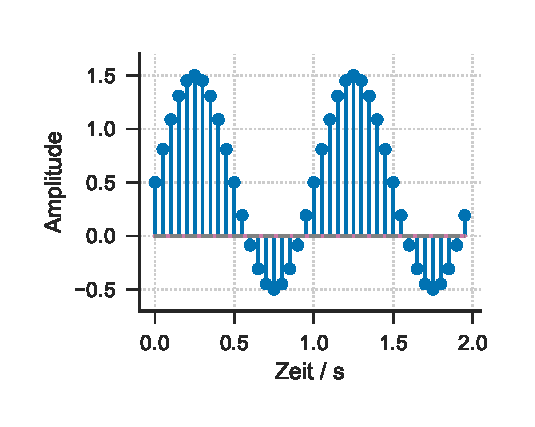
\includegraphics[scale=1]{bilder/example_signal} % oder statt scale auch [width=0.5\textwidth] für eine feste Größe
  \caption{Jede Abbildung sollte eine Bildunterschrift haben, die für sich allein aussagekräftig bleibt. Hier ist die Amplitude als Funktion von der Zeit abgebildet.}
  \label{fig:somesignal}
\end{figure}

% Emphasis, meist Kursivschrift
\emph{Hinweis}: Latex kann während der Kompilierung Tabellen und Abbildungen zur Optimierung bewegen.

\subsubsection{Gleichungen und Formeln}
Formeln können z.B. im Fließtext erscheinen: $y = 0.5 + \sin (\omega t)$. Gleichungen können aber auch in eigenen Zeilen vorkommen:
% * heißt nicht nummeriert
\begin{equation*}
    \label{simple_equation} 
    \Gamma = \gamma + \sqrt{ y } + k_0 + \frac{1}{2} \cdot x^2 + \dots
\end{equation*}

% nummerierte Gleichung
\begin{equation}
    \label{complex_equation} 
    \nabla \times \mathcal{B} = 
    \mu_0 \left( \vec{J} + \epsilon_0 \frac{\partial\vec{D}}{\partial t} \right)
\end{equation}

Mit \texttt{equation} werden die Gleichungen nummeriert und Verweise sind möglich. Das Paket \texttt{amsmath} definiert unter anderem komplexere Umgebungen, wie zum Beispiel \texttt{align}. 

% Zeilen werden getrennt durch \\ und verbunden auf &
%\begin{align}
%	a &= b + c \\ 
%   a - b &= c
%\end{align}

\subsubsection{Listen und sonstiges}
Hier ist eine Liste mit einigen allgemeinen Hinweisen, weiteren Beispielen und Links mit Tutorials:
\begin{itemize}
	\item Benutzen Sie für die Multiplikation $(a \cdot b)$ statt $(a * b)$. 
	\item In Latex schreibt man korrekterweise englische ``quotation marks'' (“ ”) bzw. deutsche "`Anführungszeichen"' („ “) -- siehe den Quellcode für Beispiele. 
	\item https://en.wikibooks.org/wiki/LaTeX/Basics
	\item https://www.sharelatex.com/learn
\end{itemize}


Ein weiteres nützliches Paket ist \texttt{siunitx}, das eine korrekte und konsistente Formatierung von Zahlen und Einheiten erzeugt. Im Quellcode finden Sie auch einige Beispiele dazu.

% $c_0 = \SI{299 792 458}{\m\per\s}$ \\
% \SI[per-mode=symbol]{1.99}[\$]{\per\kilogram}    \\
% \SI[per-mode=fraction]{1,345}{\coulomb\per\mole} \\


\vspace{1cm}
\noindent{Viel Erfolg!}